% Титульная страница — «мотив агента»: центральное ядро ИИ с лучами-руками,
% оканчивающимися глифами инструментов. Чистый вектор TikZ (адаптация оригинала;
% текст переведён на русский, рисунок сохранён).
\begin{titlepage}
\thispagestyle{empty}
\begin{tikzpicture}[remember picture, overlay]
  \fill[structurecolor] (current page.north west) rectangle ([yshift=-0.85cm]current page.north east);
  \fill[structurecolor] (current page.south west) rectangle ([yshift=0.5cm]current page.south east);
\end{tikzpicture}
\centering
\vspace*{2.5cm}

{\fontsize{32}{40}\selectfont\rmfamily\bfseries Глубокое понимание AI Agent\par}
\vspace{0.4cm}
{\Large\sffamily\color{structurecolor} Принципы проектирования и инженерная практика\par}
\vspace{0.5cm}
{\small\sffamily\color{structurecolor!70} неофициальный перевод с китайского\par}

\vspace{1.2cm}

% ── Мотив агента: центральное ядро + лучи-руки с глифами инструментов ──
\begingroup
\definecolor{ink}{RGB}{30,58,107}
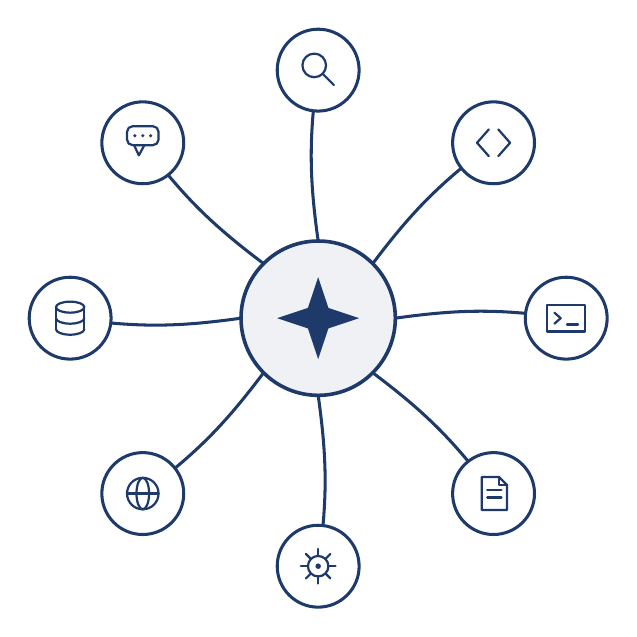
\begin{tikzpicture}[line join=round, line cap=round,
    arm/.style={ink, line width=1.1pt},
    ring/.style={ink, line width=1.1pt, fill=white},
    ic/.style={ink, line width=0.8pt}]
  \def\R{3.15}
  \def\rh{0.98}
  \foreach \a in {90,45,0,-45,-90,-135,180,135}{
    \draw[arm] (\a:\rh) to[bend left=8] (\a:\R);
  }
  \fill[ink!7] (0,0) circle (\rh);
  \draw[ink, line width=1.3pt] (0,0) circle (\rh);
  \fill[ink] (0,0.52) -- (0.13,0.13) -- (0.52,0) -- (0.13,-0.13) --
             (0,-0.52) -- (-0.13,-0.13) -- (-0.52,0) -- (-0.13,0.13) -- cycle;
  \begin{scope}[shift={(90:\R)}]
    \draw[ring] (0,0) circle (0.52);
    \draw[ic] (-0.05,0.06) circle (0.15);
    \draw[ic] (0.06,-0.05) -- (0.20,-0.19);
  \end{scope}
  \begin{scope}[shift={(45:\R)}]
    \draw[ring] (0,0) circle (0.52);
    \draw[ic] (-0.06,0.17) -- (-0.21,0) -- (-0.06,-0.17);
    \draw[ic] (0.06,0.17) -- (0.21,0) -- (0.06,-0.17);
  \end{scope}
  \begin{scope}[shift={(0:\R)}]
    \draw[ring] (0,0) circle (0.52);
    \draw[ic] (-0.24,-0.17) rectangle (0.24,0.17);
    \draw[ic] (-0.15,0.07) -- (-0.07,0) -- (-0.15,-0.07);
    \draw[ic] (0.01,-0.08) -- (0.15,-0.08);
  \end{scope}
  \begin{scope}[shift={(-45:\R)}]
    \draw[ring] (0,0) circle (0.52);
    \draw[ic] (-0.15,-0.21) -- (-0.15,0.21) -- (0.07,0.21) -- (0.17,0.11) -- (0.17,-0.21) -- cycle;
    \draw[ic] (0.07,0.21) -- (0.07,0.11) -- (0.17,0.11);
    \draw[ic] (-0.08,0.05) -- (0.10,0.05);
    \draw[ic] (-0.08,-0.05) -- (0.10,-0.05);
  \end{scope}
  \begin{scope}[shift={(-90:\R)}]
    \draw[ring] (0,0) circle (0.52);
    \draw[ic] (0,0) circle (0.13);
    \foreach \g in {0,45,90,135,180,225,270,315}{ \draw[ic] (\g:0.14) -- (\g:0.22); }
    \fill[ink] (0,0) circle (0.035);
  \end{scope}
  \begin{scope}[shift={(-135:\R)}]
    \draw[ring] (0,0) circle (0.52);
    \draw[ic] (0,0) circle (0.20);
    \draw[ic] (0,0) ellipse (0.08 and 0.20);
    \draw[ic] (-0.20,0) -- (0.20,0);
  \end{scope}
  \begin{scope}[shift={(180:\R)}]
    \draw[ring] (0,0) circle (0.52);
    \draw[ic] (0,0.14) ellipse (0.18 and 0.07);
    \draw[ic] (-0.18,0.14) -- (-0.18,-0.14);
    \draw[ic] (0.18,0.14) -- (0.18,-0.14);
    \draw[ic] (-0.18,0.0) arc[start angle=180, end angle=360, x radius=0.18, y radius=0.07];
    \draw[ic] (-0.18,-0.14) arc[start angle=180, end angle=360, x radius=0.18, y radius=0.07];
  \end{scope}
  \begin{scope}[shift={(135:\R)}]
    \draw[ring] (0,0) circle (0.52);
    \draw[ic, rounded corners=2pt] (-0.20,-0.03) rectangle (0.20,0.21);
    \draw[ic] (-0.11,-0.03) -- (-0.05,-0.16) -- (0.02,-0.03);
    \fill[ink] (-0.10,0.09) circle (0.022);
    \fill[ink] (0,0.09) circle (0.022);
    \fill[ink] (0.10,0.09) circle (0.022);
  \end{scope}
\end{tikzpicture}
\endgroup

\vfill
{\LARGE\sffamily Ли Боцзе\quad(李博杰)\par}
\vspace{0.3cm}
{\small\sffamily\color{structurecolor!80} оригинал — github.com/bojieli/ai-agent-book · Apache-2.0\par}
\vspace{0.7cm}
{\small\sffamily\color{structurecolor!80} русский перевод · v2.0 · \number\year-\number\month\par}
\vspace{1.2cm}
\end{titlepage}
